\section{Results}

\begin{figure}
\centering
\begin{tabular}{cc}
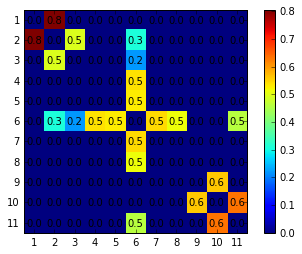
\includegraphics[width=2in]{figs/30minmin00conf} & 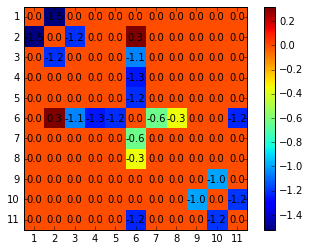
\includegraphics[width=2in]{figs/30minmin01conf} \\
(a) (0,0) & (b) (0,1) \\[6pt]
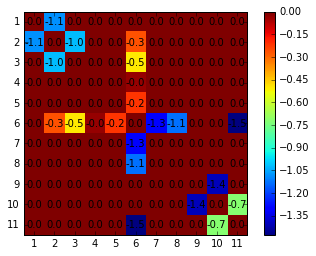
\includegraphics[width=2in]{figs/30minmin10conf} & 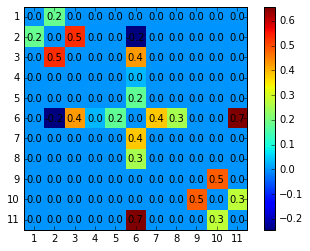
\includegraphics[width=2in]{figs/30minmin11conf} \\
(c) (1,0) & (d) (1,1) \\[6pt]
\end{tabular}
\caption{Edge potentials for the IPF run using 30 minute buckets (aggregated using \texttt{min}) in the physically connected Soda AMPlab graph (Figure~\ref{fig:physical_soda_edges}).}
\label{fig:30minminphysical}
\end{figure}

\if 0
Results:
- write it up! visualize
- we plot min/max/mean bucket at diff bucket intervals (30s, 1min 5min 10min 30min):
    - log likelihoods!
- then we interpret the highest log likelihood models:
    - fully connected
    - physically connected
\fi
